\documentclass[conference]{IEEEtran}

\usepackage{graphicx}
\usepackage{amsmath}
% \usepackage{amssym}
% \usepackage{amsthm}

\begin{document}

\title{An Exploration of Privacy and Anonymity in Bitcoin \\ {\LARGE CS203: Network and Distributed System Security}}


\author{\IEEEauthorblockN{Christopher A. Wood}
\IEEEauthorblockA{Department of Computer Science\\
University of California Irvine\\
Email: woodc1@uci.edu}
\and
\IEEEauthorblockN{Chris H. Vu}
\IEEEauthorblockA{Department of Computer Science\\
University of California Irvine\\
Email: ChrisHVu@gmail.com}}

% make the title area
\maketitle

\begin{abstract}
TODO
\end{abstract}

\IEEEpeerreviewmaketitle

\section{Introduction}
%TODO: general overview of cryptocurrency, bitcoin (why it's unique), and a summary of problems it suffers from

Electronic commerce would benefit greatly from the existence of a completely secure, private, and anonymous form of digital currency that does not rely on trusted third parties or external financial institutions to manage transactions. Motivated by this ideal type of currency, there have been many research efforts focused on generating suitable cryptography-based digital payment systems, or cryptocurrencies, such as DigiCash \cite{digicash}, E-Cash \cite{ecash}, HashCash \cite{hashcash}, Namecoin \cite{namecoin}, Peercoin \cite{peercoin}, Litecoin \cite{litecoin}, Ripple \cite{ripple}, and perhaps the most popular variant, Bitcoin \cite{bitcoin}. Each of these schemes offer different tradeoffs of security, privacy, and anonymity, and as such have varying popularity among users. However, it is the distribtued, decentralized nature of Bitcoin that has led to its widespread popularity among the general public and research communities \cite{news articles}. 

Bitcoin is distinguished from other cryptocurrencies by the fact that it does not rely on trusted third parties. Specifically, the global and publicly accessible ledger that stores records of all financial transactions, thereby serving as a verifiable history of all Bitcoin funds in circulation, is maintained by a widely distributed, peer-to-peer network of (untrusted) users. Transactions are linked to specific identities, or pseudonyms, via digital signatures used to ensure the validity of each transaction. In this context, it is often convenient to associate specific pseudonomous addresses with a single public and private key pair owned by a particular user. Unfortunately, these pseudonoyms are very weak masks for the underlying user's identity - user privacy and anonymity are still at risk even with the use of such pseudonomous identities. This is true even if a user has multiple pseudononyms and uses them with caution to deter attackers looking for such links. Consequently, user deanonymization is a major problem for Bitcoin users, and there have been several academic efforts to further the cause for Bitcoin user privacy and anonymity, including studies by Reid and Harrigan \cite{ReidHarrigan13} and Androulaki et al. \cite{Androulaki12-privacy}, and we can expect to see similar work publishing in the coming years. Elias \cite{8} also discussed some legal, and moral, aspects of the anonymity, or lack thereof, in Bitcoin. We do not focus on such legality issues here, and merely operate under the assumption that spender anonymity is an ideal property that any currency system should have.

Currently, techniques to address such anonymity issues with Bitcoin are rather limited and include the use of Chaumian's entirely independent e-cash system \cite{chaumain}, which relies on trusted third parties, and Zerocoin \cite{zerocoin}, which achieves privacy and anonymity properties based on strong cryptographic assumptions at the protocol-level by working \emph{on top of} Bitcoin, among others. The former is not ideal for several reasons; the most significant of which is that it directly conflicts with the decentralized nature of Bitcoin. The latter technique is very young, having only been published in the past year, and is just now starting to gain considerable attention \cite{pinocchio}. 

In this work we survey Bitcoin and related forms of cryptocurrency with respect to their privacy and anonymity properties. We analyze proposed solutions and offer critical insight into the open problems and difficulties in achieving perfect privacy and anonymity with minimal resource consumption (e.g., bandwidth, CPU cycles, etc.). We hope that this survey will motivate continued research on this critical problem that has the potential to change financial instutitions and forms of currency for future generations.

\todo[inline]{outline the sections here}
\section{Bitcoin Overview and Privacy Limitations}
% TODO: specific discussion of aspects of bitcoin that pertain to privacy/anonymity

TODO: intro

\subsection{Bitcoin Basics}

Bitcoin is a distributed, decentralized form of cryptocurrency. Accordingly, this enables all (digitally signed)  transactions between two parties to be conducted in a peer-to-peer fashion without the inclusion of a trusted third party, such as a bank or other financial institution. This form of decentralized exchange comes at a price, however, as there must be some way to prevent users from \emph{double spending}, or using the same funds to simultaneously pay multiple parties. Bitcoin achieves this property by relying on its users to construct a history for every transaction that takes place in the system. If a majority of the users accept the validity of a particular transaction, or a set of transactions, the global history of the system is affirmatively updated and ``confirmed'' via a cryptographic hash digest that all users agree upon. This hash digest, referred to as a hash-based proof-of-work, is what constitutes the validity of the system. By the properties of the underlying hash function, the history of the system cannot be changed without breaking the function (i.e., finding collisions) or re-doing the proof-of-work, which is computationally infeasible for small groups of nodes. Therefore, so long as a majority of the Bitcoin users are honest, the system history is deemed correct and thus all signed transactions are verified, preventing double spending by potentially malicious users participating in direct, peer-to-peer transactions. 

Unfortunately, while the above scheme is semantically correct and provides strong guarantees that all financial transactions are valid, there are inherent limitations in the amount of user privacy and anonymity that can be achieved in Bitcoin. In order to adequately define these limitations, we first describe how Bitcoin transactions are generated and how the system history is maintained. For simplicity, consider the scenario in which user $A$ wants to send $N$ BTCs (Bitcoins) to user $B$. Rather than identify users by name, Bitcoin uses \emph{addresses} that are tied to specific users to use in such transactions. Denote $\mathsf{addr}_A$ and $\mathsf{addr}_B$ as the addresses of users $A$ and user $B$ used in this transaction. It is often convenient to think of Bitcoin addresses as public keys $\mathsf{pk}_A$ and $\mathsf{sf}_B$, and as such there are corresponding private keys, which we denote as $\mathsf{sk}_A$, and $\mathsf{sk}_B$, respectively.

Structurally, a transaction $T$ is a tuple comprised of the \emph{source} transactions which supplied the funds necessary to make this transaction, denoted as $\mathsf{source}$, the (public) address of the recipient, $\mathsf{addr}_B$, the amount of BTCs to send, $N$, and a digital signature of these three properties, $\mathsf{Sign}_{\mathsf{sk_A}}({\mathsf{source}, \mathsf{pk}_B, N})$. In other words, we have 
\begin{align*}
T = (\mathsf{source}, \mathsf{pk}_B, N, \sigma), 
\end{align*}
where $\sigma = \mathsf{Sign}_{\mathsf{sk_A}}({\mathsf{source}, \mathsf{pk}_B, N})$. Note that this signature is embedded in $T$ so that any other Bitcoin user may verify the validity of the content using $\mathsf{pk}_A$. Also note that $\mathsf{source}$ need not be a single transaction; user $A$ is free to use multiple transactions in order to fund their transaction to $B$. In addition to the $N$ BTC transfer from $A$ to $B$, there is often $C$ BTC amount specified in the transaction for a particular address, where $C$ denotes the amount of change that will be given to this address as a result of the transaction. It is not required that the address to which $C$ is addressed is the same as the address of $A$, though this often happens in practice. Figure \ref{fig:transaction-io} illustrates the input and output relation of our transaction from $A$ to $B$, and Figure \ref{fig:transaction-create} illustrates the steps used in constructing this transaction. Note that, in both cases, $\mathsf{source}$ is comprised of two transactions $T_1$ and $T_2$, and the resulting transaction is denoted as $T_3$.

\begin{center}
\begin{figure}
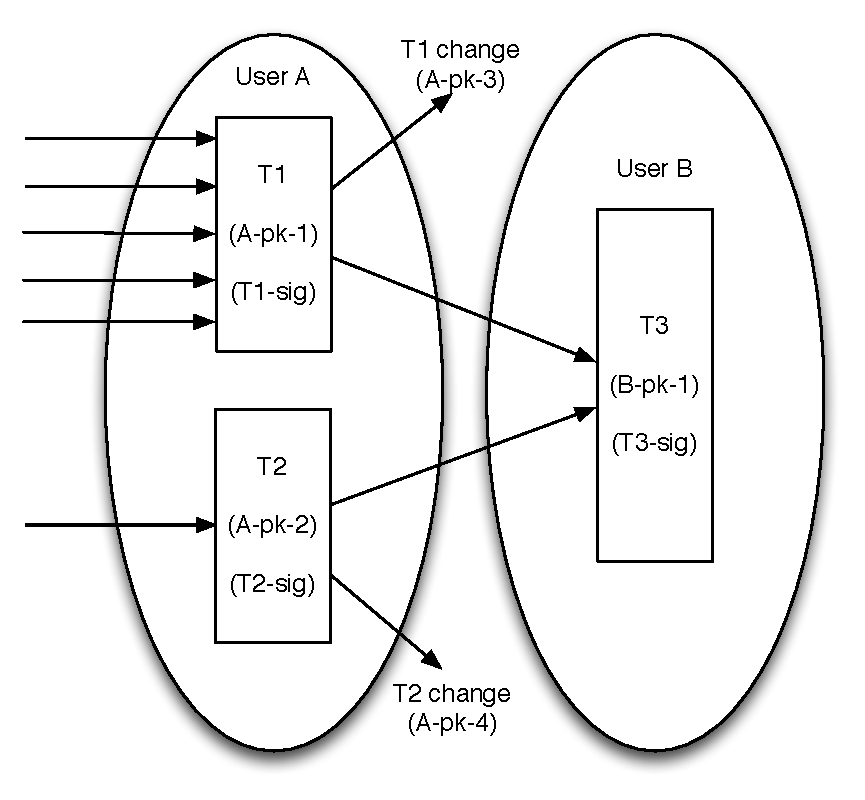
\includegraphics[scale=0.5]{./images/transaction_io.pdf}
\caption{Visual depiction of the input and output elements of a transaction from user $A$ to user $B$.}
\label{fig:transaction-io}
\end{figure}
\end{center}

\begin{center}
\begin{figure}
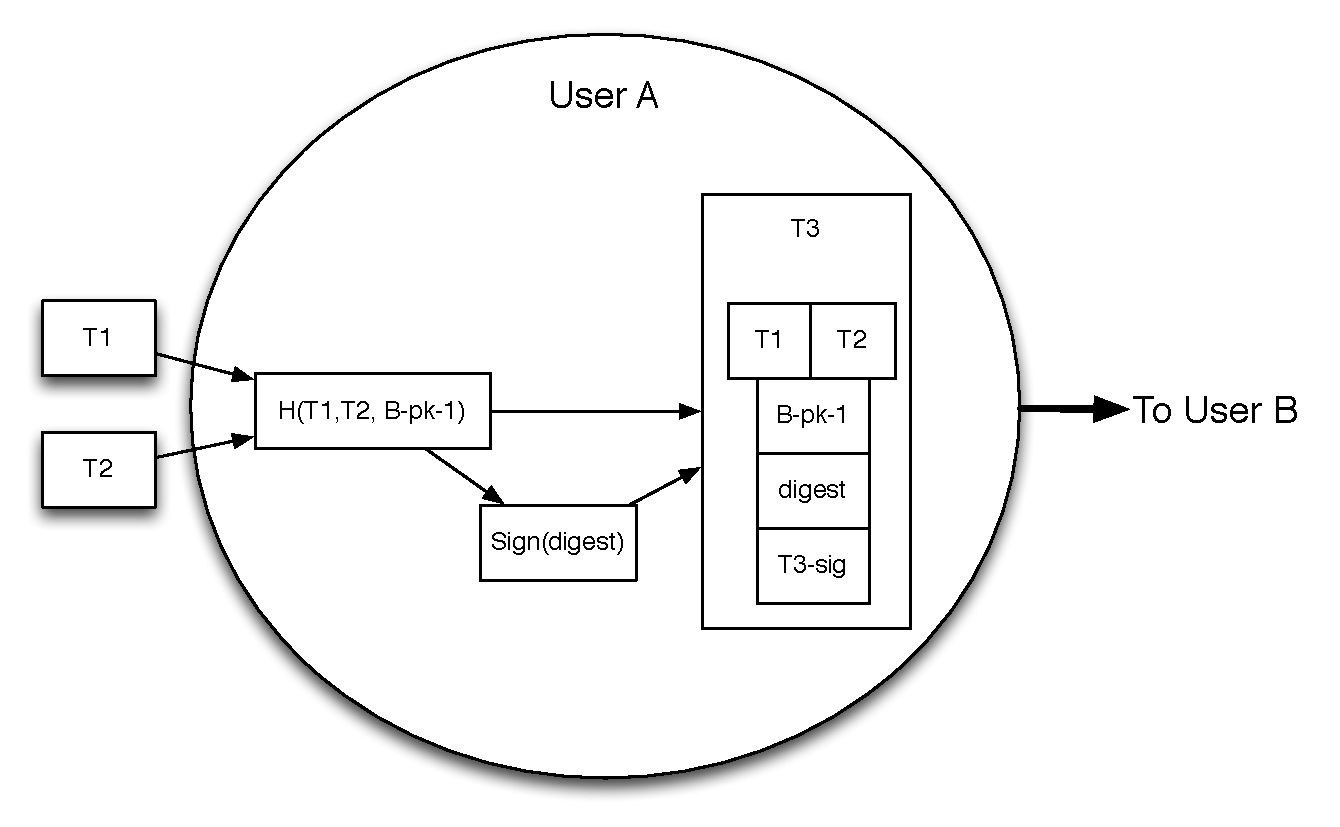
\includegraphics[scale=0.4]{./images/transaction_create.pdf}
\caption{Visual depction of the steps to create a transaction $T_3$ from user $A$ to user $B$ using two input transactions, $T_1$ and $T_2$.}
\end{figure}
\end{center}

After a transaction has been created, it is broadcasted in the network. In order to prevent double spending, nodes must confirm this transaction and append it to the chain of accepted transactions in the system's history. This procedure is based on the aforementioned proof-of-work, which works as follows. Bitcoin miners will collect unconfirmed transactions into a buffer, along with the longest chain of system-wide accepted transactions, and compute a Merkle hash of the transactions and digest of the chain. The output digest of this Merkle hash, referred to as the challenge $c$ in the proof-of-work protocol, is then used to find the proof $p$. Together, $c$ and $p$ have the property that, when concatenated and hashed using a cryptographically strong collision-resistant hash function $H$, the leading $B$ bits of the output $x = H(c || p)$ are all $0$. That is, $x = \{0,1\}^B\{0,1\}^{256-B}$. Given the collision resistant properties of $H$, finding a valid proof $p$ for the challenge $c$ is comptuationally difficult. Figure \ref{fig:block} illustrates the construction of $c$ and $p$ using a previously confirmed block chain $B$.

Once a miner finds a proof, it is broadcasted to the other nodes in the network along with the input transactions used by the miner, who can then easily recompute the challenge $c$ and verify the correctness of $p$. Once verified, this new transaction ``block'' is appended to the block chain which the miner used in finding the proof. Miners will continually use the longest block chain to gather and verify transaction blocks. Since there is a particular subset of BTCs in each transaction that are paid to the miner who provides the proof-of-work for a block containing that transaction, referred to as the transaction fee, miners are financially incentivized to collect more transactions into a block and continually ``mine'' for valid proofs-of-work. 

\subsection{Privacy Limitations}
TODO



\section{Anonymity Claims}



% 1. anonymity set size = exponential in path length
% 2. cover traffic indistinguishable from real encrypted transaction traffic


\section{Attacks, Implications, and Proposed Solutions}
\begin{itemize}
	\item transaction graph attacks
	\item passive network-layer attacks
	\item statistical attacks
\end{itemize}

%Vu - I may switch attack on privacy with anonymity and have anonymity first.  Need to reconcile user-network graphs and transaction-network graphs with attacks on privacy and anonymity.

\subsection{Attacks on Privacy}
%Current loss of privacy through voluntary identification/off network information, flow analysis, IP tracking. Needs more info
As a currency system, Bitcoin cannot have perfect privacy. Although the information originates outside the Bitcoin network, some address ownership information are public knowledge. For instances, a store needs to have a publicly identifiable address in order to accept payment for goods or services.  Users may also disclose address ownership when asking for donations or posting on Bitcoin forums [6]. Large centralized Bitcoin services such as the Mt. Gox exchange service are also able to associate users with addresses as part of their service.

The trivial attack on privacy involve using the Bitcoin block chain to follow all the transactions associated with that address. As user commonly have many addresses, a more sophisticated attack requires the adversary to link the known address with other hidden addresses and then analyze the transactions associated with those addresses. The two major heuristics for linking addresses are \emph{multi-address transactions} and \emph{shadow or change addresses}. 

Multi-address transactions are transactions with more than one source. Currently, Bitcoin allows for users to use more than one source address in a transaction, but does not allow multiple users to pay for one transaction. For example, suppose $\mathsf{addr}_A$ has 3 Bitcoins (BTC) and $\mathsf{addr}_B$ has 2 BTC. The user uses both addresses to pay 4 BTC to $\mathsf{addr}_C$ and puts the remainder of 1 BTC to $\mathsf{addr}_D$. Only one user can be the input to any transaction, therefore in this example, $\mathsf{addr}_A$ and $\mathsf{addr}_B$ belong to the same user.

\emph{Shadow addresses} or \emph{change accounts} are accounts created for change from a transaction. In the transaction above, $\mathsf{addr}_D$ is the shadow account that belongs to the same user that controls $\mathsf{addr}_A$ and $\mathsf{addr}_B$. Although not directly related to the Bitcoin system, the way Bitcoin clients handle shadow accounts can break address indistinguishability [4]. However, because shadow accounts rely on user behavior instead of an inherent property of the Bitcoin system, the shadow account heuristic is not as robust [6].

Using these two heuristics, researchers have been able cluster addresses with a common owner in a user graph where every node is a user and every edge is a transaction [5][6][7]. In any node where the user has revealed ownership of an address, the user's privacy has been lost.

Another privacy loss channel is the TCP/IP layer. As previously mentioned, Bitcoin uses a peer-to-peer network to transmit transactions. Many services, such as Bit Faucet, will log and publish the IP address of users of the service. A more active attack would include malicious nodes scanning for Bitcoin clients listening to port TCP/8333 [7] and open a direct connection. While proxy services like Tor can hide outbound connections, an inbound connection will not be obfuscated. By listening to transaction announcements over time, the client that first reports a transaction is the one that initiated it. This allows the malicious nodes to link transactions to IP addresses.

\subsection{Attacks on Anonymity}
%should we combine this with the privacy section?
%attacks on address indistinguishabiilty include multi-address transactions and shadow/change accounts
Researchers attempt to break the anonymity of Bitcoins in an attempt to study stolen Bitcoins [6][8]. In a similar manner to the attack on privacy, a user graph is created. 
%There is research between big data (the user and transaction graphs) and re-identifying people. Netflix and social networks (Broken Promise of Privacy: Responding to the Surprising Failure of Anonymization by Paul Ohm and De-anonymizing Social Networks by Arvind Narayanan and Vitaly Shmatikov).  Is this outside the scope of our paper? It's alluded that user transaction graphs can be used to identify real world identities, but no one has done it yet.


\subsection{Current and Proposed Solutions}
%Centralized mixes similar to Chaums anonymous email (BitFog, BitLaundry, Blockchain.info) and decentralized mixes (Zerocoin).

%[5]Dorit Ron and Adi Shamir. Quantitative Analysis of the Full Bitcoin Transaction Graph. IACR Cryptology ePrint Archive 584 (2012).

%[6] Sarah Meiklejohn, Marjori Pomarole, Grant Jordan, Kirill Levchenko, Damon McCoy, Geoffrey M. Voelker, and Stefan Savage. 2013. A fistful of bitcoins: characterizing payments among men with no names. In Proceedings of the 2013 conference on Internet measurement conference(IMC '13). ACM, New York, NY, USA, 127-140

%[7] Fergal Reid and Martin Harrigan. 2013. An Analysis of Anonymity in the Bitcoin System. Security and Privacy in Social Networks. Springer, New York, NY, USA, 197-223

%[8] Dan Kaminsky. 2011. Black Ops of TCP/IP 2011. Black Hat USA 2011. http://www.slideshare.net/dakami/black-ops-of-tcpip-2011-black-hat-usa-2011

%[9] Malte Moser. 2013. Anonymity of Bitcoin Transactions: An Analysis of Mixing Services. Munster Bitcoin Conference (MBC). July 17-18, Munster, Germany
\section{Fundamental Problems and New Ideas} \label{sec:open}

Based on our review of the literature, it is quite clear that Bitcoin is far from being a completely anonymous form of currency. Before first attempting to derive such a currency, it is important to explicitly capture what it means for a currency system to provide its users anonymity.Ideally, an anonymous form of (digital) currency would have the following properties:
\begin{enumerate}
	\item Users should be able to validate the monetary value associated with a coin (or bill) without learning any additional information. This is akin to validating the monetary value of a \$20 dollar bill found on the ground - one cannot determine (with reasonable effort) where the bill came from or who previously owned said bill. 
	\item The system should enable users to possess coins without learning who owns what coins. Using the dollar metaphor, this is again similar to the case where the any person is able to acquire and spend bills as they see fit, but the US treasury and other people are not able to see what bills are owned by a specific user unless they attempt to make a payment. 
	\item Users should be able to prove ownership of a coin without revealing their identity. 
\end{enumerate}

Enumerating the goals in this manner makes it quite easy to see why the Zerocoin extension to Bitcoin is such a natural solution to anonymous currency. Zerocoin supports all three properties through cryptographic techniques such as accumulators and zero knowledge proofs of knowledge, which, when used according to the protocol, enable coins to be spent anonymously. Recall that Zerocoin achieves this through the use of a virtual ``bulliten board'' of transaction committments, where the value of a transaction is verified by churning out the result of an accumulator and the proof of ownership is done via a zero-knowledge proof of knowledge of the secret information needed to reveal \emph{one} committment on the bulliten board. However, the development of Pinocchio Coin \cite{pinocchio} to enhance the Zerocoin protocol with alternative cryptographic primitives that yield the same behavior is an indication that this anonymity comes at a price. Furthermore, since these techinques are more sophisticated than native Bitcoin protocol ``operations,'' the chance of an implementation or engineering error leading to an exploitable side channel through which to conduct a deanonymization attack is greatly increased. 

Such risks may be unavoidable, however, as even the next-best, low-cost, natively supported solutions for anonymity in Bitcoin (e.g., mixing services) do not provide perfect anonymity. In particular, while mixing serices may bend and break the links in transaction graph, masking the original generator of a particular transaction, compromised services can still lead to client input and output information leakage if implemented poorly. 

To date, we believe that Zerocoin is the most popular form of completely anonymous currency proposed. While it is still too early to tell whether or not Zerocoin will see widespread adoption. However, reports indicate that the first Zerocoins will become available in May 2014 \cite{zerocoin-press}. Until then, it may still be worthwhile to investigate alterantive means for creating anonymious currency. We now propose one such idea: Suppose that instead of transactions being associated with a single sender, they were associated with a group of $k$ users. That is, each transaction was signed by $k$ distinct users using some aggregate signature technique \cite{aggrsig1}. Among this set of $k$ users there exists exactly one user who is the generator of the transaction, but the members of the group cannot identify said user. This property can be achieved by having the single generating user $U$ send the transaction $T$ to each member of the group using the Dining Cryptographer's Protocol \cite{dining}. This protocol enables $U$ to multicast $T$ to the other $k-1$ members of the group with \emph{complete information-theoretic anonymity}. When $T$ has been retrieved by all $k$ users, they would then engage in an aggregate signature computation over $T$ before broadcasting it to the rest of the network. Alternatively, one single user may inject a \emph{group signature} in $T$ where the verification key is associated with the $k$ users. This approach has the drawback that $k$-size groups must be predefined and keys must be carefully managed. 

Observe that, if the transaction $T$ is distributed throughout the $k$-group using an anonymity-preserving protocol, then the anonymity set of the transaction is effectively $k$, the set of all users who participate in the aggregate (or group) signature. Based on prior transaction graph analysis attacks, this would help circumvent deanonymization attacks on single users based on transaction clustering. Of course, this property comes at the cost of efficiency, as the communication and computation complexity of performing an anonymous multicast and aggregate signature is quite high depending on the particular techniques used. If, however, nodes can spare these cycles and network resources, this may be a viable solution worth pursuing. 

% idea: assign each transaction a k-bit ID, and then have small clusters perform DC protocol k times to send transactions to everyone in the cluster, and then when done, every node in that cluster broadcasts the transaction -> |T| determines complexity of the approach
% 	-> when broadcasted, the cluster ID (or set of addresses) is included in the transaction, anonymity set is the size of the cluster
% 	-> hides who originally created the transaction
% 	-> analogous to a group securely generating a new transaction, as opposed to a single user
% 	-> group performs aggregate signature after the message has been transmitted and appends that to the transaction

% - downside: mixing services help break the link from transaction graph, but compromised services can still lead to leaking information about client inputs and client outputs (engineering limitation)
% - plusside: can be built using existing protocol
% - plusside: Zerocoin doesnt suffer from that implementation problem
% - downside: not supported, needs to be a new form of cryptocurrency, or use Bitcoin or something else as backing currency 
% - downside: computationlal complexity and increased liklihood of error

% \begin{itemize}
% 	\item need to unlink transactions from users - this is an inherent problem that comes with the block chain
% 	\item transaction graph essentially serves as a means for people to check whether or not the funds for an address were at some point transferred to that address -> this is why ZK proofs as digital committments and accumulators are such an intuitive solution
% \end{itemize}



\section{Related Cryptocurrencies} \label{sec:related}
Although Bitcoin is inarguably the most popular cryptocurrency to date, it is by no means the first such technology proposed. Other popular variants include DigiCash \cite{digicash}, E-Cash \cite{ecash}, HashCash \cite{hashcash}, Namecoin \cite{namecoin}, Peercoin \cite{peercoin}, Litecoin \cite{litecoin}, and Ripple \cite{ripple}. In this section we briefly describe some of these variants with respect to their anonymity properties. Our discussion begins with E-Cash \cite{ecash}.

Chaum, Fiat, and Naor’s offered two methods to create untraceable electronic cash. Both methods require a central bank organization. In all methods, the coins that are issued by the bank are blinded in a way to prevent the bank from identifying the source of honestly spent coins. The first method uses “untraceable coins” in that each transaction is of set amounts. Alice creates random commitments and sends them to the bank. The bank uses a subset of those commitments to create cryptographic coins by signing them. The bank then sends those coins to Alice after decrementing the amount from Alice’s account.  Everyone can verify the coin’s structure and the bank’s signature. Alice can then spend those coins to pay Bob. To do so, Alice sends Bob the information on the coin as well as a zero-knowledge proof that Alice initiated the creation of the coin. When Bob tries to redeem the coin with the bank, Bob sends both pieces of information to the bank. The bank will not have enough information to identify the coin came from Alice unless Alice tries to double spend. In that case, there is a high probability one of the challenges in the zero-knowledge proofs from the merchants will be different allowing the bank to reconstruct Alice’s identity. This method underpins the DigiCash system.

\begin{figure}
\begin{center}
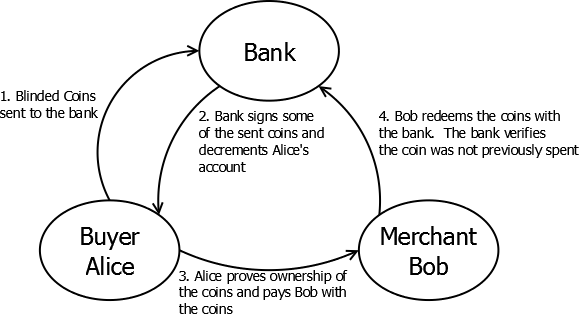
\includegraphics[scale=0.30]{images/digicash.png}
\caption{Digicash protocol.}
\label{fig:tor-end-to-end}
\end{center}
\end{figure}

The second method outlined is ``untraceable checks''.  The idea builds upon the “untraceable coins” idea by giving Alice has a roll of coins.  Alice can spend them by indexing the roll of coins by the purchase amount and revealing that to the merchant.  Alice is then refunded the rest of the amount by the bank by creating a separate transaction to pay herself.

Compact E-Cash builds upon the framework that Chaum creates with Untraceable Electronic Cash by creating a coin that can be used repeatedly a limited number of times. The system is comprised of a “withdrawal protocol”, a “spending protocol”, and a “double spending” check.  The withdrawal protocol involves the user creating a private key as well as the coin’s serial number and blinding value. The bank then signs the values and decrements the user’s account accordingly. The spending protocol has the user give the merchant the coin’s serial number, the merchant’s random number challenge, and a double-spending value based on the user’s private key, the random number challenge, and the blinding value.  The user also gives the merchant two non-interactive proofs.  The first proof is that the committed coin was signed by the bank.  The second proof verifies that the coin’s serial number and double spending number correspond to the commitment as well. The merchant then reveals this information to the bank for payment. In order to protect the user’s privacy, the serial number that is revealed to the merchant is encrypted using the user’s private key. In order to prevent the user from cheating, if the same coin is used over the limited number of uses, the bank is able to infer the secret key of the user, decrypt the serial number of the coin, and identify the user. This also means that the user can re-use coins a number of times without the bank being able to identify the user.
 
The Compact E-Cash system allows for users to create coins that can be used multiple times. The coins do not reveal the spending habits of the user if the user does not try to cheat and re-use the same coin too many times. The drawbacks are that there must be a central bank to issue coins and verify transactions. Also, each time a coin is used is a separate transaction even if the user spends multiple coins with the same merchant.

In both systems, privacy is maintained by blinded coins. If the user uses the system honestly and does not double spend, then the bank cannot reveal the identity of the user based on the coins used. Furthermore, because the coins are indistinguishable, the bank is unable to create profiles based on the location the coins were spent.

A mature form of the “untraceable coins” is the Mondex Smart Card. The bank issues secure cards embedded with an integrated circuit. The cards store “value” on the card. The “value” is incremented when money is transferred onto the card and decremented when the card is used for payment or deposit. In essence, if Alice pays Bob 5 coins, Alice’s card will destroy 5 coins and Bob’s card will create 5 coins. This makes the individual coins impossible to track. However, both Alice and Bob’s cards will have a transaction ledger that ties Alice’s and Bob’s cards to the transaction. Similar to a Bitcoin address, the card provides limited privacy as it separates the user from the coins being spent. However, merchants are able to create purchasing profiles based on transaction logs and the card’s internal identification. Furthermore, the system does not prevent merchants from sharing purchasing information with the issuing bank to match card identification numbers with an identity. In this way, the Mondex Smart Card system is less anonymous than other cryptocurrencies and does not provide any guarantees of privacy.

HashCash was originally designed to stop the waste or abuse of internet resources. HashCash requires the actor, Alice, to provide a proof-of-work before allowing an action such as sending an email. The idea is to add a cost to the action to prevent abuse. HashCash now has been incorporated into Bitcoin and similar cryptocurrency systems in the mining process as the proof-of-work protocol, but is not used as a currency system by itself. There are three protocols and two public variables in the original interactive HashCash system. The public variables are a hash function, $H(\cdot)$, and the length parameter $w$. In the Challenge protocol, the server, Bob, sends Alice the service name $s$ and a random challenge value $c$. Alice runs the Mint protocol to run a brute-force search for the value $x$. The hash of $s|c|x$, where $|$ represents concatenation, creates a value with $w$ leading zeroes. After Alice sends $x$ to Bob, Bob runs the Verify protocol to verify Alice’s work. If Verify succeeds, Alice is allowed to perform her action using the requested service. HashCash improvements include replacing the service name and challenge with a fixed output string and requiring Alice to find a collision. The proof-of-work can be considered a currency as it is used to create a transaction. If used in this way, HashCash does provide slightly better privacy than Bitcoins. Proofs-of-work are public knowledge, but HashCash does not have a ledger and therefore new nodes do not have access to the history of work.

\begin{figure}
\begin{center}
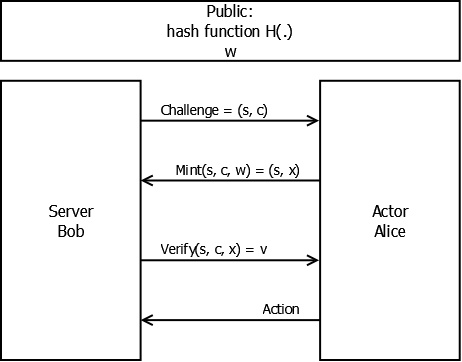
\includegraphics[scale=0.40]{images/hashcash.png}
\caption{Hashcash protocol.}
\label{fig:tor-end-to-end}
\end{center}
\end{figure}

Other alternative cryptocurrencies are based off the Bitcoin system, but only Zerocoin increases privacy. The other systems do not improve or reduce the privacy as compared to Bitcoin. Litecoin is the most similar to Bitcoin as it only differs in a few aspects. The first difference is that Litecoin uses scrypt instead of SHA-256, which is used in Bitcoin. Second, Litecoin has faster block times which decreases the time needed for a transaction confirmation. Finally, Litecoin increases the total number of coins available to be mined. Peercoin combines the HashCash proof-of-work method of mining coins with a second method, proof-of-stake. Proof-of-stake uses the notion of coin age. The coin age of a wallet is the sum of the lengths of time since a coin’s previous transaction. If Alice received 4 coins 2 days ago, then her wallet’s coin age would be 8 coin-days. In proof-of-stake, one hash per unspent wallet-output is created each second. Whereas the proof-of-work protocol uses a fixed hash target, proof-of-stake uses a variable hash target that scales inversely with coin age. If Alice finds an accepted value, she creates a transaction paying herself and is awarded one percent of her transaction as a reward. Being that her coins were used in a transaction, the mining process resets the coin age of Alice’s wallet. Namecoin is a cryptocurrency based off Bitcoin in the sense that the coins are used to register and transfer domain names. Namecoin is designed as a decentralized DNS. The ledger, which already contains coin transactions, will also contain DNS transactions such as the creation or purchase of a domain name and the associated IP address.

Unlike the previous cryptocurrencies which are based on the transference of “value”, Ripple is based on the transference of “debt”. Ripple is comprised of two parts. The first part involves a web-of-trust between nodes. Alice determines how much she trusts Bob and Charlie and then extends the maximum debt she is willing to accept from them. Suppose Charlie owes Alice 5 coins and Alice wanted to pay Bob 5 coins, but Bob only trusts Alice with a debt of 2 coins. If Bob trusts Charlie with a debt of 3 coins, Alice can send an IOU for 2 coins from her and an IOU for 3 coins from Charlie. Bob receives an IOU totaling 5 coins from which he can collect from Alice and Charlie at a later date or use to make payments to someone else.

\begin{figure*}[ht]
\begin{center}
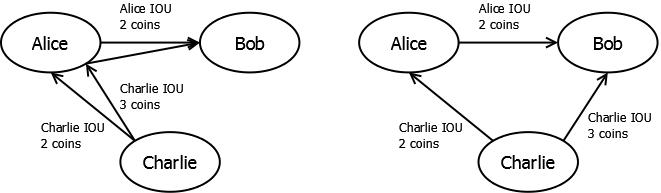
\includegraphics[scale=0.40]{images/ripple.png}
\caption{Ripple debt network.}
\label{fig:tor-end-to-end}
\end{center}
\end{figure*}

The second part of Ripple is to facilitate transactions where no web-of-trust exists. This is done through “gateway” nodes. Gateways act as publically known trusted nodes analogous to banks. If Alice wanted to pay Bob 5 coins, but Bob only trusts a gateway, then Alice can send 5 coins to the gateway and the gateway will credit Bob 5 coins. Unlike the first part of Ripple, gateways use stores of “value” instead of debt. Ripple is as private as Bitcoins as transfers of debt or credit between addresses is public knowledge, but no registry ties addresses to people. The exception is if Ripple deals with real world currency. Ripple is currency agnostic and therefore gateways are free to use real world currency as an exchange medium. In this case, gateways require personal information from the user and are able to link users to addresses and transactions.


\section{Conclusion}
In this survey we provided an extensive study of the anonymity properties of Bitcoin. We discussed all known attacks published in scholarly literature, elaborated on possible solutions to improve anonymity, and also discussed potential avenues for future work. We also briefly discussed related cryptocurrencies to provide some reference against which Bitcoin can be compared.

\begin{thebibliography}{1}

\bibitem{bitcoin} Satoshi Nakamoto. Bitcoin: A Peer-to-Peer Electronic Cash System. \emph{Consulted} 1 (2008).

\bibitem{chaumain} David Chaum. Blind Signatures for Untraceable Payments. \emph{Crypto} 82 (1982).

\bibitem{zerocoin} Ian Miers, Christina Garman, Matthew Green, Aviel D. Rubin. Zerocoin: Anonymous Distributed E-Cash from Bitcoin. \emph{IEEE Symposium on Security and Privacy} (2013).

\bibitem{Androulaki12-privacy} Elli Androulaki, Ghassan O. Karame, Marc Roeschlin, Tobias Scherer, and Srdjan Capkun. Evaluating User Privacy in Bitcoin. \emph{IACR Cryptology ePrint Archive} 596 (2012).

\bibitem{Shamir13-bitcoingraph} Dorit Ron and Adi Shamir. Quantitative Analysis of the Full Bitcoin Transaction Graph. \emph{IACR Cryptology ePrint Archive} 584 (2012).



%%% @Vu: put your bib entries here and cite them using \cite{item-name}, e.g., \cite{bitcoin} (References the first entry above)

\end{thebibliography}




% that's all folks
\end{document}


